

%!TEX root = /Users/kevin/SkyDrive/KTH Work/Period 3 2014/DN2255/Homework/1/Heat Equation/Heat Equation.tex
\section{Numerical results} 

% (fold)
\label{sec:numerical_results}
\begin{enumerate}
	\item \textbf{Solution plots: Show plots of the solution for some time levels before and after t = 1/4, for \textbf{both} source functions S.} 
	
	{\color{blue} Figures~\ref{fig:Figures_deltaFunctionPlot} and \ref{fig:Figures_exponentialFunctionPlot} are plots of the solution with a delta function and Gaussian function, Equation~\eqref{eq:sourceFunction}, as source terms. For both of these plots, space discretization was $m=n=100$ and time discretization was $dt=1e-4$ seconds.} 
	\begin{figure}
		[htbp] \centering 
		\includegraphics[width=
		\textwidth]{Figures/deltaFunctionPlot.eps} \caption{Results with a delta function at the center as a source.} \label{fig:Figures_deltaFunctionPlot} 
	\end{figure}
	
	% (fig:Figures_deltaFunctionPlot)
	\begin{figure}
		[htbp] \centering 
		\includegraphics[width=
		\textwidth]{Figures/exponentialFunctionPlot.eps} \caption{Results with Equation~\eqref{eq:sourceFunction} as the source function.} \label{fig:Figures_exponentialFunctionPlot} 
	\end{figure}% (fig:Figures_exponentialFunctionPlot)
	
	\item \textbf{Convergence }
	\item \textbf{Numerical Conservation}: Demonstrate that the method is numerically conservative by looking at 
	\begin{equation}
		\int q \mathrm{~d}x \mathrm{d}y = \Delta x \Delta y \sum Q_{ij} \label{eq:numConservation} 
	\end{equation}% (eq:numconservation)
\begin{figure}
	[htbp] \centering 
	\subfigure[Source - Delta Function at center]{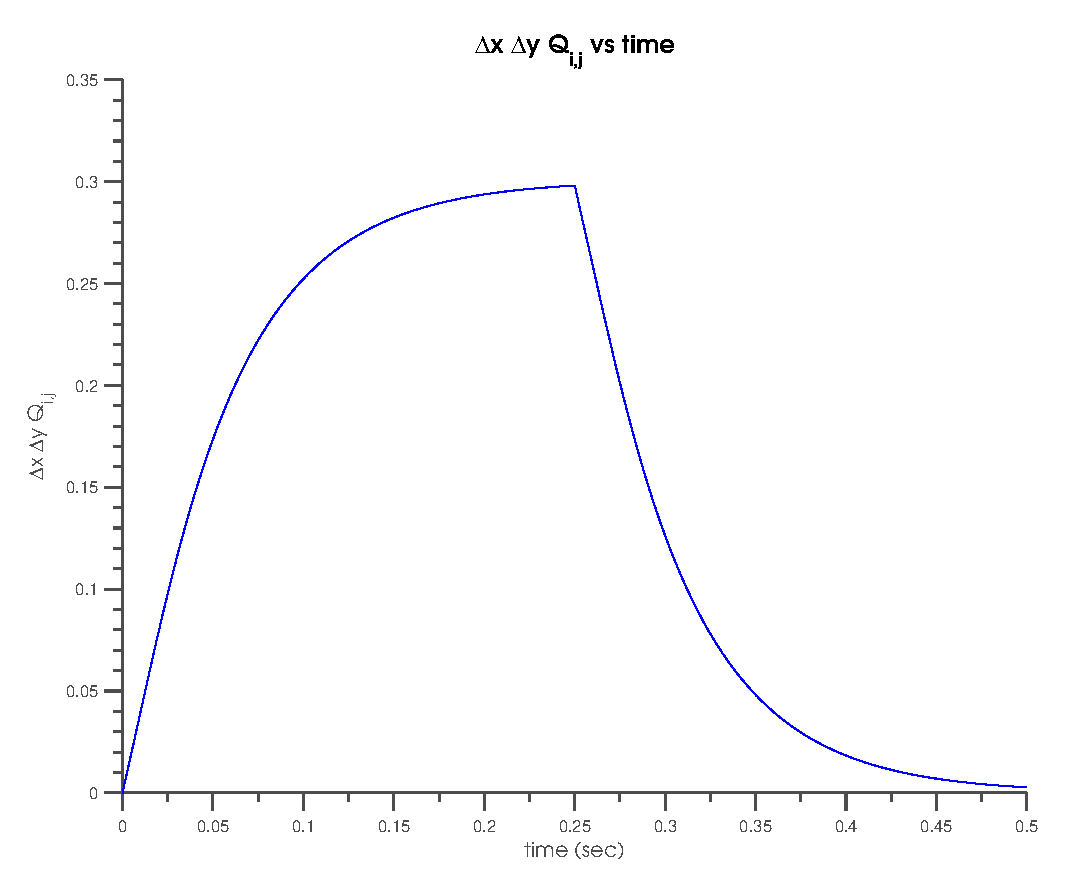
\includegraphics[width=.48\textwidth]{Figures/deltaConservationPlot.eps} \label{fig:deltaConservationPlot}} % (subfigure 1)
	\subfigure[Source - Gaussian Distribution at center]{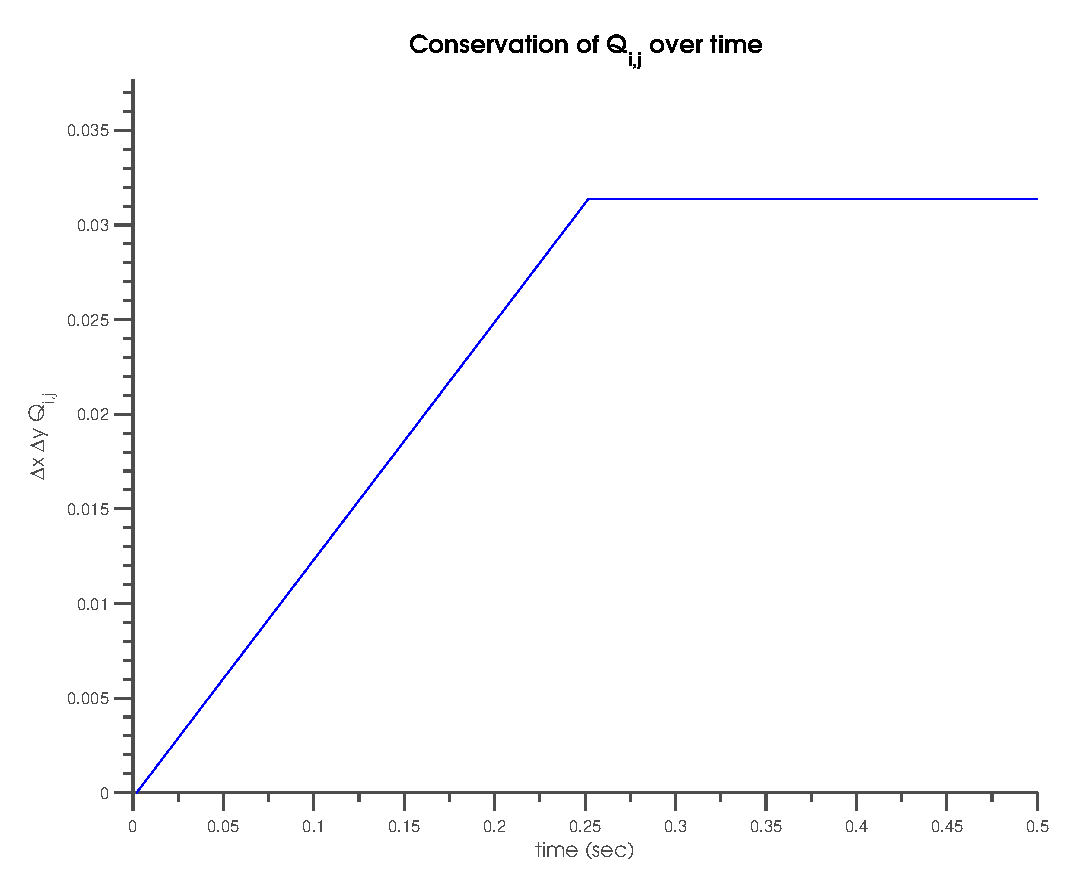
\includegraphics[width=.48\textwidth]{Figures/sourceConservationPlot.eps} \label{fig:sourceConservationPlot}} % (subfigure 2)
	\caption{Plot of Equation~\eqref{eq:numConservation} to show conservation of the quantity $Q_{i,j}$ over time.  The plot has a source term adding heat to the system, but after $t=0.25~s$, the source is shut off and the amount of Q does not change over time.}
\end{figure} % (fig:Figures_fronttrackingfig4)

	\begin{itemize}
		\item[i.] \textbf{Time-discretization and how your code handles the discontinuity in g(t)}
		
		{\color{blue} My code handles the discontinuity in g(t) by using two loops with the first loop including the source term and going from $t=0$ to $t= ts \cdot \tau$ where $ts=\mathrm{round}(0.25/\tau)$.} 
		\item[ii.] \textbf{Space-discretization; where in the cell does (x,y)=(1/2,1/2) appear? different for odd and even m,n}
		
		{\color{blue} The cell (1/2, 1/2) appears only for odd values of m,n and is at $(m+1)/2$. For example, if $m=n=11$, then $(x_{6},y_{6}) = (1/2,1/2)$.} 
	\end{itemize}
\end{enumerate}

% section numerical_results (end)
